\documentclass[journal]{IEEEtran}
\usepackage[a5paper, margin=10mm, onecolumn]{geometry}
\usepackage{lmodern}
\usepackage{tfrupee}
\setlength{\headheight}{1cm}
\setlength{\headsep}{0mm}

\usepackage{gvv-book}
\usepackage{gvv}
\usepackage{cite}
\usepackage{amsmath,amssymb,amsfonts,amsthm}
\usepackage{algorithmic}
\usepackage{graphicx}
\usepackage{textcomp}
\usepackage{xcolor}
\usepackage{txfonts}
\usepackage{listings}
\usepackage{enumitem}
\usepackage{mathtools}
\usepackage{gensymb}
\usepackage{comment}
\usepackage[breaklinks=true]{hyperref}
\usepackage{tkz-euclide}
\usepackage{listings}
\def\inputGnumericTable{}
\usepackage[latin1]{inputenc}
\usepackage{color}
\usepackage{array}
\usepackage{longtable}
\usepackage{calc}
\usepackage{multirow}
\usepackage{hhline}
\usepackage{ifthen}
\usepackage{lscape}
\usepackage{xparse}

\bibliographystyle{IEEEtran}

\title{9.5.6}
\author{EE25BTECH11043 - Nishid Khandagre}

\begin{document}
\maketitle

\renewcommand{\thefigure}{\theenumi}
\renewcommand{\thetable}{\theenumi}

\numberwithin{equation}{enumi}
\numberwithin{figure}{enumi}

\textbf{Question}:
Find the sum and product of the roots of the quadratic equation 
\begin{align*}
2x^2-9x + 4 = 0
\end{align*}

\textbf{Solution:}
Given quadratic equation:
\begin{align}
    y=2x^2 - 9x + 4
\end{align}
Representing this equation as a conic section
\begin{align}
    \vec{x}^{\top}\vec{V}\vec{x} + 2\vec{u}^{\top}\vec{x} + f=0 \ , \  \vec{V}=\myvec{2 & 0\\0&0} \ , \  \vec{u}=\myvec{-9/2 \\ -1/2} \ ,\ f=4
\end{align}
We need to find intersection points with $y=0$, that is, the X-axis.
\begin{align}
    \vec{x}=\vec{h} + k \vec{m} \ , \ \vec{h}=\myvec{0 \\ 0} \ , \ \vec{m}=\myvec{1 \\ 0}
\end{align}
Substituting $\vec{x} = k \vec{m}$
\begin{align}
    k^2\vec{m}^{\top}\vec{V}\vec{m} + 2k\vec{u}^{\top}\vec{m} + f=0 \\
    \implies k= \dfrac{1}{2 \vec{m}^{\top}\vec{V}\vec{m}} \sbrak{ -2\vec{u}^{\top}\vec{m} \ \pm \ \sqrt{\brak{2\vec{u}^{\top}\vec{m}}^2 - 4 f \vec{m}^{\top}\vec{V}\vec{m}}}\\
    \implies k= \dfrac{1}{\vec{m}^{\top}\vec{V}\vec{m}} \sbrak{ -\vec{u}^{\top}\vec{m} \ \pm \ \sqrt{\brak{\vec{u}^{\top}\vec{m}}^2-f \vec{m}^{\top}\vec{V}\vec{m}}}\\
    \vec{u}^{\top}\vec{m} = \myvec{-9/2 & -1/2}\myvec{1 \\0} = -9/2 \\
    \vec{m}^{\top}\vec{V}\vec{m}=\myvec{1 & 0}\myvec{2 & 0\\0&0}\myvec{1 \\ 0} = 2\\
    k= \dfrac{1}{2} \sbrak{ -\brak{-9/2} \ \pm \ \sqrt{ \brak{-9/2}^2 - 4 \cdot 2}}\\
    k= \dfrac{1}{2} \sbrak{ \dfrac{9}{2} \ \pm \ \dfrac{7}{2}}\\
    \implies k_1= 4\\
    \implies k_2= \dfrac{1}{2}
\end{align}
Substituting $k$ into $\vec{x}$, we get the roots:
\begin{align}
    \vec{x} = \myvec{4 \\ 0} \text{ OR } \vec{x}=\myvec{1/2 \\ 0}
\end{align}
This implies that the roots of $2x^2 -9x + 4 =0$ are $4$ and $\frac{1}{2}$.

Now, calculate the sum and product of these roots:\\
Sum of the roots:
\begin{align}
\text{Sum} = 4 + \frac{1}{2} = \frac{9}{2}
\end{align}
Product of the roots:
\begin{align}
\text{Product} = 4 \times \frac{1}{2} = 2
\end{align}

\begin{figure}[H]
\centering
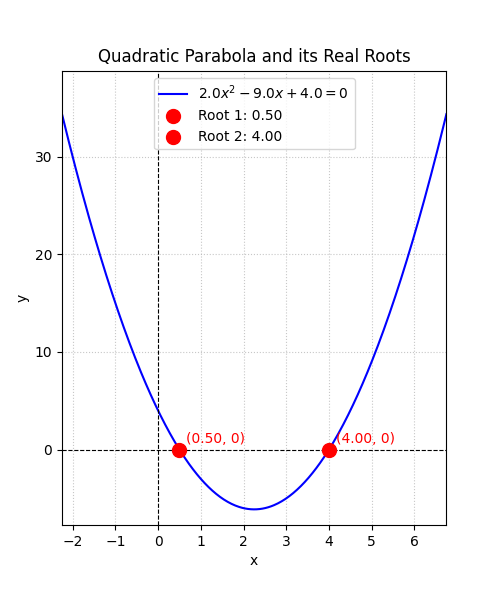
\includegraphics[width=0.7\columnwidth]{figs/fig1.png}
\caption{}
\label{fig:1}
\end{figure}

\end{document}
